\documentclass[10.5pt,letterpaper]{article}

% ---------- Core packages ----------
\usepackage[T1]{fontenc}
\usepackage[utf8]{inputenc}
\usepackage{lmodern}
\usepackage[margin=1in,top=1.15in,bottom=1.15in]{geometry}
\usepackage{xcolor}
\usepackage{titlesec}
\usepackage{titletoc}
\usepackage{fancyhdr}
\usepackage{enumitem}
\usepackage{tabularx}
\usepackage{booktabs}
\usepackage{colortbl}
\usepackage{array}
\usepackage[most]{tcolorbox}
\usepackage{tikz}
\usetikzlibrary{shapes.geometric,positioning,arrows.meta,fit,backgrounds,calc}
\usepackage{parskip}
\usepackage[hidelinks,pdfusetitle]{hyperref}
\usepackage{multicol}
\usepackage{ragged2e}

% ---------- Brand palette (matches the product's Aurora indigo/cyan theme) ----------
\definecolor{brandIndigo}{HTML}{4F46E5}
\definecolor{brandIndigoDark}{HTML}{1E1B4B}
\definecolor{brandCyan}{HTML}{0EA5E9}
\definecolor{brandViolet}{HTML}{8B5CF6}
\definecolor{brandSlate}{HTML}{334155}
\definecolor{brandSlateLight}{HTML}{64748B}
\definecolor{brandBgGray}{HTML}{F8FAFC}
\definecolor{brandBorder}{HTML}{E2E8F0}
\definecolor{brandGreen}{HTML}{059669}
\definecolor{brandAmber}{HTML}{D97706}

% ---------- Section styling ----------
\titleformat{\section}
  {\normalfont\Large\bfseries\color{brandIndigoDark}}
  {\colorbox{brandIndigo}{\makebox[2.2em]{\color{white}\thesection}}}
  {0.6em}{}
\titlespacing*{\section}{0pt}{1.6em}{0.9em}

\titleformat{\subsection}
  {\normalfont\large\bfseries\color{brandIndigo}}
  {\thesubsection}{0.6em}{}
\titlespacing*{\subsection}{0pt}{1.2em}{0.5em}

\titleformat{\subsubsection}
  {\normalfont\normalsize\bfseries\color{brandSlate}}
  {\thesubsubsection}{0.5em}{}
\titlespacing*{\subsubsection}{0pt}{1em}{0.35em}

% ---------- Headers / footers ----------
\pagestyle{fancy}
\fancyhf{}
\renewcommand{\headrulewidth}{0.4pt}
\renewcommand{\footrulewidth}{0.4pt}
\fancyhead[L]{\small\color{brandSlateLight}\textsf{resume-forge}}
\fancyhead[R]{\small\color{brandSlateLight}\textsf{Technical White Paper}}
\fancyfoot[L]{\small\color{brandSlateLight}\textsf{\textcopyright\ 2026 --- Confidential}}
\fancyfoot[R]{\small\color{brandSlateLight}\textsf{Page \thepage\ of \pageref{LastPage}}}
\usepackage{lastpage}

\fancypagestyle{plain}{%
  \fancyhf{}
  \renewcommand{\headrulewidth}{0pt}
  \fancyfoot[L]{\small\color{brandSlateLight}\textsf{\textcopyright\ 2026 --- Confidential}}
  \fancyfoot[R]{\small\color{brandSlateLight}\textsf{Page \thepage\ of \pageref{LastPage}}}
}

% ---------- Reusable boxes ----------
\newtcolorbox{statbox}[1]{
  colback=brandBgGray, colframe=brandBorder, boxrule=0.6pt, arc=3pt,
  left=10pt, right=10pt, top=8pt, bottom=8pt, title={#1},
  fonttitle=\bfseries\color{brandIndigoDark}\normalsize,
  coltitle=brandIndigoDark
}

\newtcolorbox{calloutbox}[1][]{
  enhanced, colback=white, colframe=brandIndigo, boxrule=0pt,
  leftrule=3pt, arc=0pt, outer arc=0pt,
  left=11pt, right=11pt, top=7pt, bottom=7pt, #1
}

\newtcolorbox{securitybox}{
  enhanced, colback=white, colframe=brandGreen, boxrule=0pt,
  leftrule=3pt, arc=0pt, outer arc=0pt, left=11pt, right=11pt, top=7pt, bottom=7pt
}

\newcommand{\metric}[2]{%
  \begin{minipage}[t]{0.235\textwidth}
    \centering
    {\fontsize{22}{24}\selectfont\bfseries\color{brandIndigo}#1}\\[2pt]
    {\small\color{brandSlateLight}\textsf{#2}}
  \end{minipage}%
}

% ---------- Misc ----------
\setlist[itemize]{leftmargin=1.35em, itemsep=3pt, topsep=4pt, label=\textcolor{brandIndigo}{\textbullet}}
\setlist[enumerate]{leftmargin=1.5em, itemsep=3pt, topsep=4pt}
\renewcommand{\arraystretch}{1.25}
\setlength{\parindent}{0pt}

\title{resume-forge}
\author{}
\date{}

\begin{document}

% ============================================================= TITLE PAGE
\begin{titlepage}
\newgeometry{margin=0in}
\begin{tikzpicture}[remember picture, overlay]
  \fill[brandIndigoDark] (current page.north west) rectangle (current page.south east);
  \shade[top color=brandIndigo, bottom color=brandIndigoDark, opacity=0.55]
    (current page.north west) rectangle ([yshift=-9.5cm]current page.north east);
  \fill[brandCyan, opacity=0.18] ([shift={(3.2cm,-3.5cm)}]current page.north west) circle (3.4cm);
  \fill[brandViolet, opacity=0.20] ([shift={(-2.5cm,-6.2cm)}]current page.north east) circle (3.0cm);
  \draw[brandCyan, opacity=0.5, line width=1.1pt]
    ([yshift=-9.6cm]current page.north west) -- ([yshift=-9.6cm]current page.north east);
\end{tikzpicture}

\vspace*{2.1cm}
\begin{center}
  {\sffamily\small\color{brandCyan!85!white}\MakeUppercase{Technical White Paper}}\\[0.55cm]
  {\sffamily\fontsize{40}{44}\selectfont\bfseries\color{white}resume-forge}\\[0.35cm]
  {\sffamily\Large\color{white!85!brandIndigoDark}Local-First, LLM-Powered Resume Tailoring}\\[0.15cm]
  {\sffamily\Large\color{white!85!brandIndigoDark}with Deterministic ATS Scoring}\\[1.6cm]
  {\sffamily\normalsize\color{white!70!black}
    Core Library \quad\textbullet\quad
    Web Application \quad\textbullet\quad \\[4pt]
    MCP Server \quad\textbullet\quad
    Command-Line Interface}
\end{center}

\vspace{4.3cm}
\begin{center}

\begin{tikzpicture}
  \node[draw=white!40!brandIndigo, rounded corners=2pt, line width=0.8pt,
        text=white, inner sep=10pt, minimum width=9.5cm]
   {\begin{tabular}{@{}ll@{}}
      \textsf{\textbf{Version}} & \textsf{1.0 --- Feature-Complete Release} \\[4pt]
      \textsf{\textbf{Date}} & \textsf{July 2026} \\[4pt]
      \textsf{\textbf{Classification}} & \textsf{Internal / Project Documentation} \\[4pt]
      \textsf{\textbf{Repository}} & \textsf{github.com/vishalVasanthakumarPoornima/}\\
       & \textsf{Resume-Tailor-ATS-Scorer}
    \end{tabular}};
\end{tikzpicture}
\end{center}

\vfill
\begin{center}
  {\sffamily\footnotesize\color{white!65!black}
   Prepared as project documentation for resume-forge --- an open-source,
   privacy-preserving resume tailoring system.}
\end{center}
\vspace{1cm}
\restoregeometry
\end{titlepage}
\setcounter{page}{1}

% ============================================================= TOC
\pagestyle{plain}
\tableofcontents
\thispagestyle{plain}
\newpage
\pagestyle{fancy}

% ============================================================= EXEC SUMMARY
\section*{\textcolor{brandIndigoDark}{Executive Summary}}
\addcontentsline{toc}{section}{Executive Summary}

resume-forge is a full-stack system that tailors a candidate's resume to a specific job
posting, scores the result against a deterministic, transparent model of an Applicant
Tracking System (ATS), and iterates automatically until a target score is met --- all while
mechanically guaranteeing that no employer, degree, certification, or skill is ever invented.
The system is delivered as four cooperating interfaces built on one shared core: a Python
library, a web application, a Model Context Protocol (MCP) server for agentic integration,
and a command-line tool.

The defining engineering decision in this project is \textbf{provider independence for
inference}. Rather than binding the product to a single LLM vendor, resume-forge implements
a pluggable backend layer that auto-detects the best available option at runtime: a free-tier
cloud model (z.ai/GLM, Google Gemini, Groq, or Puter) when a credential is present, or a fully
local Ollama model with zero external dependency otherwise. This yields a system that runs
identically whether the operator has no API budget at all, a free-tier key, or an enterprise
subscription to Anthropic's Claude --- with cloud inference reducing per-run latency from
minutes to seconds.

\begin{center}
\begin{tcolorbox}[colback=brandBgGray, colframe=brandBorder, boxrule=0.6pt, arc=3pt,
  left=6pt,right=6pt,top=10pt,bottom=10pt, width=\textwidth]
\centering
\metric{4}{Product Interfaces}
\metric{8}{Pipeline Stages}
\metric{94}{Automated Tests}
\metric{7}{LLM Backends}
\end{tcolorbox}
\end{center}

This document describes the problem resume-forge solves, its architecture and data-integrity
guarantees, its scoring methodology, its multi-provider inference strategy, its security and
privacy posture, and the quality assurance process behind it.

\newpage

% ============================================================= 1. INTRODUCTION
\section{Introduction and Problem Statement}

\subsection{The Applicant Tracking System Problem}
The overwhelming majority of mid-size and large employers filter inbound resumes through an
Applicant Tracking System before a human ever sees them. These systems parse résumé text,
match it against keyword and skill taxonomies extracted from the job requisition, and rank or
reject candidates algorithmically. A resume that is a strong substantive match for a role can
still be filtered out for entirely mechanical reasons: a non-standard section header, a
graphics-heavy template that fails text extraction, a multi-column layout that scrambles
reading order, or simply an absence of the specific terminology the posting uses.

\subsection{Why Manual Tailoring Fails to Scale}
The standard advice --- ``tailor your resume to every job'' --- is sound but expensive. A
candidate applying to twenty roles in a search would need to manually re-read each posting,
identify its priority keywords, and rewrite bullet content to surface the right prior
experience in the right language, without ever crossing the line into embellishment or
fabrication. This is slow, inconsistent under fatigue, and difficult to self-audit: a
candidate under pressure to hit a keyword target has a natural incentive to stretch the truth,
whether intentionally or not.

\subsection{Design Goals}
resume-forge was built against four non-negotiable requirements:

\begin{enumerate}
  \item \textbf{Never fabricate.} Tailoring must be limited to emphasis, reordering, and
    rewording of facts already present in the candidate's master resume. This must be
    enforced in code, not merely requested in a prompt.
  \item \textbf{Score against a real, inspectable model of ATS behavior}, not a black box ---
    so the candidate can see exactly why a resume did or did not clear a threshold and what
    to do about it.
  \item \textbf{Run without a paid API dependency}, so cost is never a barrier to iterating on
    a job search, while still allowing an upgrade path to faster or higher-quality inference
    when available.
  \item \textbf{Be usable four ways}: interactively via a browser, programmatically as a
    Python library, as a tool an AI agent can call (MCP), and as a scriptable CLI --- so it
    composes with other tooling rather than being a dead-end application.
\end{enumerate}

\newpage

% ============================================================= 2. SOLUTION OVERVIEW
\section{Solution Overview}

resume-forge accepts two inputs --- an existing resume (PDF, DOCX, \LaTeX, or plain text) and
a job posting (a URL or pasted text) --- and produces a tailored, compiled, single-page PDF
resume together with a numeric ATS compatibility score, a breakdown of that score by
dimension, and a list of concrete, truthful improvements still available. An optional
grounded cover letter can be generated in the same pass.

\begin{statbox}{What Makes This Different}
\begin{itemize}
  \item \textbf{Structural fabrication guard.} Tailored output is diffed against the
    candidate's verified master profile using fuzzy entity matching; any employer or
    institution the model invents is discarded, and any the model omits is
    \emph{automatically restored} from the source of truth.
  \item \textbf{Deterministic scorer.} The ATS score is computed by plain Python --- regular
    expressions, section detection, and weighted keyword coverage --- not by asking an LLM to
    grade its own work.
  \item \textbf{One-page guarantee.} The \LaTeX\ rendering pipeline enforces single-page,
    single-sided output through progressive spacing compaction rather than truncating
    content.
  \item \textbf{Provider-agnostic inference.} The same pipeline runs unmodified on a free
    cloud API, a paid frontier model, or a fully offline local model.
\end{itemize}
\end{statbox}

\subsection{End-to-End Flow}
\begin{enumerate}
  \item The candidate's master resume is parsed once into a structured profile
    (contact, summary, skills, experience, projects, education, certifications) and cached
    by content hash, so repeated runs against the same resume skip re-parsing entirely.
  \item The job posting is fetched (or accepted as pasted text) and extracted into a
    structured requirements object: title, company, required skills, preferred skills,
    keywords, and responsibilities.
  \item The tailoring stage rewrites and reorders the master profile's content to match the
    posting's language, under a hard no-fabrication instruction enforced both in the prompt
    and in a post-processing guard.
  \item The tailored content is rendered into an ATS-friendly \LaTeX\ template and compiled to
    PDF.
  \item The compiled PDF is scored by the local, deterministic ATS scorer.
  \item If the score is below the target, the scorer's specific feedback --- missing
    keywords, weak subscores --- is fed back into the tailoring stage, and steps 3--5 repeat,
    up to a configurable iteration cap.
  \item The best-scoring result across all iterations is returned, together with the full
    score report, even if the target was never reached.
\end{enumerate}

\newpage

% ============================================================= 3. ARCHITECTURE
\section{System Architecture}

\subsection{Four Interfaces, One Core}
resume-forge is deliberately layered so that the tailoring logic is written exactly once and
consumed four different ways.

\begin{center}
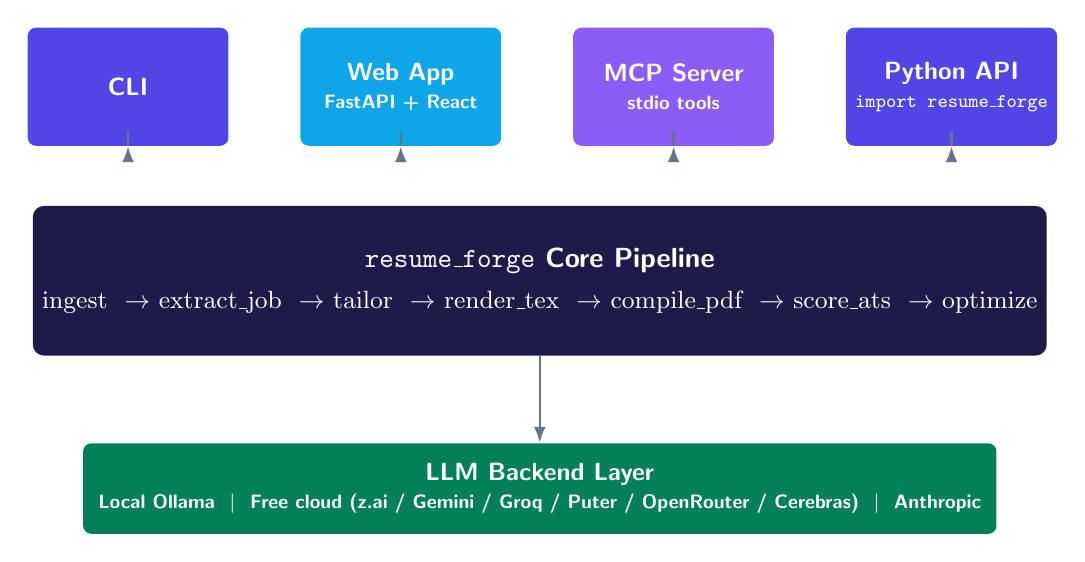
\begin{tikzpicture}[
  node distance=0.55cm and 0.9cm,
  layer/.style={rectangle, rounded corners=3pt, minimum width=2.55cm, minimum height=1.5cm,
    align=center, font=\sffamily\small\bfseries, text=white, draw=none},
  core/.style={rectangle, rounded corners=4pt, minimum width=11.6cm, minimum height=1.9cm,
    align=center, font=\sffamily\normalsize\bfseries, text=white, fill=brandIndigoDark, draw=none},
  lbl/.style={font=\sffamily\scriptsize, text=brandSlateLight}
]
  \node[layer, fill=brandIndigo] (cli) {CLI};
  \node[layer, fill=brandCyan, right=of cli] (web) {Web App\\[-1pt]{\scriptsize FastAPI + React}};
  \node[layer, fill=brandViolet, right=of web] (mcp) {MCP Server\\[-1pt]{\scriptsize stdio tools}};
  \node[layer, fill=brandIndigo, right=of mcp] (api) {Python API\\[-1pt]{\scriptsize \texttt{import resume\_forge}}};

  \node[core, below=0.75cm of $(cli.south)!0.5!(api.south)$] (core)
    {\texttt{resume\_forge} Core Pipeline\\[3pt]
     \small\normalfont ingest \ $\rightarrow$\ extract\_job \ $\rightarrow$\ tailor \ $\rightarrow$\
     render\_tex \ $\rightarrow$\ compile\_pdf \ $\rightarrow$\ score\_ats \ $\rightarrow$\ optimize};

  \foreach \n in {cli,web,mcp,api}{ \draw[-{Latex[length=2mm]}, brandSlateLight, line width=0.8pt] (\n.south) -- ([yshift=0.75cm]core.north -| \n.south); }

  \node[layer, fill=brandGreen!85!black, below=1.1cm of core, minimum width=11.6cm, minimum height=1.15cm]
    (backend) {LLM Backend Layer\\[-1pt]{\scriptsize Local Ollama\ \ $\vert$\ \ Free cloud (z.ai / Gemini / Groq / Puter / OpenRouter / Cerebras)\ \ $\vert$\ \ Anthropic}};
  \draw[-{Latex[length=2mm]}, brandSlateLight, line width=0.8pt] (core.south) -- (backend.north);
\end{tikzpicture}
\end{center}

\subsection{Layer Responsibilities}
\begin{tabularx}{\textwidth}{@{}l X@{}}
\toprule
\rowcolor{brandIndigoDark}
\textcolor{white}{\textbf{Layer}} & \textcolor{white}{\textbf{Responsibility}} \\
\midrule
\textbf{Core library} & Every pipeline stage as an independently testable, pure(ish) Python
  function with Pydantic-validated inputs and outputs. No interface-specific logic lives
  here. \\
\rowcolor{brandBgGray}
\textbf{Web application} & FastAPI backend running jobs on a background thread with live
  per-stage progress; a React + Vite + Tailwind frontend with animated, branded UI
  components. Ships in a single-process production mode. \\
\textbf{MCP server} & Exposes \texttt{tailor\_resume}, \texttt{extract\_job\_posting},
  \texttt{score\_resume}, and \texttt{ingest\_resume} as Model Context Protocol tools over
  stdio, so any MCP-aware agent (including other Claude-based projects) can call the
  pipeline directly. \\
\rowcolor{brandBgGray}
\textbf{CLI} & A thin \texttt{argparse} wrapper (\texttt{resume-forge}) for scripted or
  terminal use, supporting stdin piping for job descriptions. \\
\bottomrule
\end{tabularx}

\newpage

% ============================================================= 4. PIPELINE DEEP DIVE
\section{Pipeline Deep Dive}

Every stage below is an independently importable, independently tested function in the
\texttt{resume\_forge} package.

\subsection{Stage 1 --- Resume Ingestion}
The master resume (PDF via \texttt{pdfplumber}, DOCX via \texttt{python-docx}, or plain
text/\LaTeX) is extracted to text and parsed once by the LLM into a structured
\texttt{MasterProfile}: contact information, summary, categorized skills, work experience
with dated bullets, projects, education, and certifications. The result is cached to disk
keyed by a hash of the file's bytes, so identical resumes are never re-parsed.

\begin{calloutbox}
\textbf{Reliability guard.} Small or quantized language models occasionally return a
schema-valid but empty parse (Section~6.3 explains why). resume-forge detects a suspiciously
empty result against a non-trivial resume, retries once with a corrective prompt, and --- on
Ollama specifically --- escalates to the strongest locally installed model as a last resort
before failing loudly. It never silently returns an empty resume.
\end{calloutbox}

\subsection{Stage 2 --- Job Extraction}
A job posting URL is fetched with a single polite \texttt{httpx} request and its main content
extracted with \texttt{trafilatura} (BeautifulSoup as fallback). If that fails --- common on
job boards that block automated access --- resume-forge falls back to an optional headless
Chromium render (Playwright) for JavaScript-rendered postings, and finally to
directly-pasted text. The result is parsed into required skills, preferred skills, general
keywords, and responsibilities.

\subsection{Stage 3 --- Tailoring}
The master profile and job requirements are given to the LLM under an explicit hard rule
(reproduced in full in Section~6) that tailoring means only emphasis, reordering, and
rewording of existing facts. Output is a \texttt{TailoredResume} of the same shape as the
master profile.

\subsection{Stage 4 --- \LaTeX\ Rendering}
Tailored content is rendered into a Jinja2-templated \LaTeX\ document using
\texttt{\textbackslash VAR\{\}}/\texttt{\textbackslash BLOCK\{\}} delimiters (chosen so the
delimiters themselves are valid \LaTeX\ and do not collide with document syntax). All
user-derived text passes through a dedicated escaping filter that handles both the seven
\LaTeX\ special characters and Unicode punctuation (em/en dashes, curly quotes, ellipses)
that would otherwise silently disappear under T1 font encoding.

\subsection{Stage 5 --- PDF Compilation}
The \LaTeX\ source is compiled with \texttt{tectonic}, a self-contained \TeX\ engine that
fetches packages on demand, with \texttt{pdflatex} as a fallback if tectonic is unavailable.
Compiler errors are parsed and surfaced as a focused log excerpt rather than a raw dump.

\subsection{Stage 6 --- ATS Scoring}
The compiled PDF's text is extracted and scored by a fully local, deterministic model of ATS
behavior. Full methodology in Section~7.

\subsection{Stage 7 --- Optimization Loop}
If the score is below target, the scorer's missing keywords and weakest subscores are fed
back into Stage 3 as structured feedback, and Stages 3--6 repeat up to a configurable
iteration cap (default 5). The no-fabrication guarantee holds on every iteration --- a
keyword the master profile cannot truthfully support will simply remain missing, and the
final report says so explicitly rather than pretending otherwise.

\subsection{Stage 8 --- Optional Cover Letter}
When requested, a grounded cover letter is generated under the same fabrication contract: the
model writes body paragraphs only, while the salutation, date, and signature are assembled
from verified data. Placeholder tokens and stray sign-offs are stripped programmatically as a
second line of defense.

\newpage

% ============================================================= 5. LLM STRATEGY
\section{Multi-Provider Inference Strategy}

\subsection{The Problem With Binding to One Provider}
Any tool that hard-codes a single LLM vendor inherits that vendor's cost structure, rate
limits, and availability as its own. resume-forge instead treats the LLM as a swappable
component behind a two-method protocol (\texttt{parse(system, prompt, output\_type) ->
output\_type}), with every backend returning schema-validated, Pydantic-typed output.

\subsection{Supported Backends}
\begin{tabularx}{\textwidth}{@{}l l l X@{}}
\toprule
\rowcolor{brandIndigoDark}
\textcolor{white}{\textbf{Backend}} & \textcolor{white}{\textbf{Cost}} &
\textcolor{white}{\textbf{Latency}} & \textcolor{white}{\textbf{Notes}} \\
\midrule
z.ai (GLM) & Free tier & Seconds & Default auto-detected cloud backend; \texttt{glm-4.5-flash}
  / \texttt{glm-4.7-flash} genuinely free, not trial credit \\
\rowcolor{brandBgGray}
Google Gemini & Free tier & Seconds & Largest free daily quota of the supported providers \\
Groq & Free tier & Seconds & Fastest raw inference speed observed \\
\rowcolor{brandBgGray}
Puter & Free (token) & Seconds & Resells GLM and other models with no z.ai account
  required; one free Puter token \\
OpenRouter / Cerebras & Free tier & Seconds & Additional free-tier options with presets \\
\rowcolor{brandBgGray}
Generic OpenAI-compatible & Varies & Varies & Escape hatch for any compatible endpoint,
  including keyless self-hosted servers \\
Ollama (local) & Free & Tens of seconds & Fully offline; zero external dependency; used
  automatically when no cloud credential is present \\
\rowcolor{brandBgGray}
Anthropic (Claude) & Paid & Seconds & Opt-in only; never auto-selected, since it is the
  only backend with a direct cost \\
\bottomrule
\end{tabularx}

\subsection{Selection Logic}
At startup, resume-forge resolves the active backend in strict priority order: an explicit
\texttt{--backend} flag or \texttt{RESUME\_FORGE\_LLM\_BACKEND} environment variable wins
outright; otherwise the system scans, in order, for a present API key among the free cloud
providers and auto-selects the first one found; if none is present, it falls back to a local
Ollama model with no configuration required at all. Anthropic is deliberately excluded from
auto-detection so that a stray credential in the environment never causes an unexpected
charge.

\begin{securitybox}
\textbf{Local-first fallback.} Because the local Ollama path requires zero credentials and
zero network access, resume-forge is guaranteed to run in a fully air-gapped environment.
Cloud backends are a latency optimization layered on top of that guarantee, never a
requirement.
\end{securitybox}

\subsection{Structured Output on Constrained Local Models}
A significant engineering finding from this project concerns Ollama's grammar-constrained
JSON decoding: it emits object keys in \emph{schema declaration order} and can only skip
optional keys, never revisit them. A source document (such as a resume) presenting
information in a different order than the schema --- for example, listing education before
work experience --- caused the model to silently omit every field ``before'' the point it
began writing, producing a schema-valid but substantively empty parse. The fix, now applied
unconditionally, marks every property in every object of the JSON schema as required before
it is sent to the model, eliminating the entire failure class. This was verified by
side-by-side testing on the same malformed input before and after the fix.

\newpage

% ============================================================= 6. NO-FABRICATION
\section{Data Integrity: The No-Fabrication Guarantee}

\subsection{Why a Prompt Alone Is Not Enough}
Instructing a model not to fabricate is necessary but not sufficient --- language models can
still drift, omit, or subtly reword a fact into something false, especially under a
smaller or quantized model. resume-forge treats this as a systems problem, not a prompting
problem, and enforces the guarantee at three independent layers.

\subsection{Layer 1 --- The Explicit Rule}
Every tailoring and cover-letter prompt embeds the following instruction verbatim:

\begin{calloutbox}
\itshape\small
``Only use facts present in the master profile. NEVER invent or alter employers, job
titles, employment dates, degrees, institutions, GPAs, certifications, project names, or
metrics. Every number in a bullet must already exist in the master profile. Tailoring means
emphasis, reordering, rewording, and keyword alignment --- NOT adding experience the
candidate does not have. If the job asks for a skill the candidate lacks, simply do not
mention it; do not imply familiarity.''
\end{calloutbox}

\subsection{Layer 2 --- The Structural Guard}
After every tailoring call, the output is programmatically diffed against the master
profile using fuzzy entity matching (canonicalized string comparison plus similarity
scoring) that tolerates harmless cosmetic drift --- ``Perficient, Inc.'' matching
``Perficient'' --- while still catching genuine fabrication:
\begin{itemize}
  \item Any employer, project, or certification in the tailored output that does not
    fuzzy-match an entry in the master profile is \textbf{removed}.
  \item Any employer or education entry present in the master profile but
    \textbf{omitted} by the model is \textbf{restored} --- tailoring can structurally never
    delete a candidate's employment history.
  \item Education entries are copied verbatim from the master profile without exception;
    rewording a degree (for example, rephrasing an in-progress program as completed) is a
    correctness risk with no offsetting benefit.
  \item Contact information is always taken from the verified profile, never from model
    output, with a regex-based backfill recovering fields (email, phone, LinkedIn, GitHub)
    that a smaller model sometimes drops during parsing.
\end{itemize}

\subsection{Layer 3 --- Truthful Keyword Backfill}
Conversely, if the model over-trims a skill that genuinely exists in the master profile and
is also requested by the job posting, it is restored into the tailored skills section. This
ensures the optimization loop can close truthful keyword gaps without the fabrication guard
fighting against legitimate emphasis.

\begin{statbox}{Net Effect}
The tailored resume is provably a strict subset of facts already present in the candidate's
verified master profile, rearranged and reworded for relevance --- with any additions to,
or omissions from, either direction reconciled automatically against the source of truth.
\end{statbox}

\newpage

% ============================================================= 7. SCORING
\section{ATS Scoring Methodology}

\subsection{Design Philosophy}
Rather than asking an LLM to self-grade the resume it just wrote --- an approach vulnerable
to reward hacking and inconsistent grading --- resume-forge scores the \emph{compiled PDF's
extracted text} with plain, deterministic Python. This mirrors how a real ATS operates: it
never sees the source \LaTeX\ or the model's intent, only what a PDF text extractor can pull
out of the finished document.

\subsection{Weighted Dimensions}
\begin{tabularx}{\textwidth}{@{}l c X@{}}
\toprule
\rowcolor{brandIndigoDark}
\textcolor{white}{\textbf{Dimension}} & \textcolor{white}{\textbf{Weight}} &
\textcolor{white}{\textbf{What It Measures}} \\
\midrule
Keyword coverage & 40 & Weighted match rate against the job's required and preferred
  skills and general keywords; required skills weigh double preferred/general terms \\
\rowcolor{brandBgGray}
Parseability & 15 & Clean text extraction from the PDF --- penalizes embedded-font
  artifacts, encoding replacement characters, and unusually low text density per page \\
Standard sections & 15 & Presence of conventional headers (Experience, Education, Skills)
  that ATS parsers are tuned to recognize \\
\rowcolor{brandBgGray}
Bullet quality & 15 & Fraction of content lines beginning with a strong action verb and
  fraction carrying a quantified result (a number, percentage, or dollar figure) \\
Contact information & 10 & Machine-detectable email address and phone number \\
\rowcolor{brandBgGray}
Length & 5 & Page count and total word count within a reasonable range for the format \\
\midrule
\textbf{Total} & \textbf{100} & \\
\bottomrule
\end{tabularx}

\subsection{Output}
Every scoring call returns the overall score, the six subscores against their maxima, the
specific keywords still missing (required-weight keywords sorted first), and a list of
actionable, plain-English suggestions --- all of which feed the optimization loop's next
tailoring attempt.

\newpage

% ============================================================= 8. ONE-PAGE RENDERING
\section{Resume Rendering and the One-Page Guarantee}

\subsection{Template Design}
The \LaTeX\ template is deliberately conservative for ATS compatibility: single column,
standard fonts, no graphics, no tables used for content layout (only for genuinely tabular
data), and real selectable text throughout. This is the same category of layout choice that
most professional ATS-optimization guidance recommends, applied structurally rather than
left to chance.

\subsection{Guaranteeing a Single, Single-Sided Page}
Rather than truncating content to force a page break --- which risks silently dropping a
qualification --- the renderer applies a sequence of \emph{progressively compact} spacing
presets (margin, line spacing, section spacing, and bullet spacing) and re-compiles until the
result fits one page, only reducing content as a last resort and never removing a full
section. This preserves substance while producing the tight, professional density that both
human recruiters and ATS parsers expect from a one-page resume.

\newpage

% ============================================================= 9. SECURITY
\section{Security and Privacy}

\begin{securitybox}
\textbf{No inbound network exposure.} The web application binds to \texttt{127.0.0.1} by
default and is intended for local, single-user use. Job state is held in-process; nothing is
persisted to an external service.
\end{securitybox}

\subsection{Data Handling}
\begin{itemize}
  \item The candidate's resume never leaves the machine except as the prompt payload sent to
    whichever LLM backend is active --- and when that backend is local Ollama, it never
    leaves the machine at all.
  \item API credentials are read from a local, git-ignored \texttt{.env} file and are never
    logged, echoed, or transmitted anywhere other than the configured provider's own API
    endpoint.
  \item Job-posting scraping performs a single polite HTTP request per attempt with a
    standard browser user agent --- no login automation, no CAPTCHA or bot-wall evasion, and
    no retry hammering. Sites whose Terms of Service prohibit automated access (several major
    job boards among them) are expected to block the request; the documented and supported
    fallback is for the user to paste the posting text directly.
\end{itemize}

\subsection{File System Boundaries}
All model-supplied file paths (in the text-editor-style tool surfaces used during
development and testing) are canonicalized and verified to remain within the intended
project root before any read or write, rejecting path traversal via \texttt{..} sequences,
symlinks, or encoded variants.

\newpage

% ============================================================= 10. QA
\section{Quality Assurance and Testing}

\subsection{Test Suite}
resume-forge ships with a fully offline, fully mocked automated test suite --- no network
access and no live LLM calls are required to run it. As of this release, \textbf{94 tests
pass}, covering:

\begin{multicols}{2}
\begin{itemize}
  \item ATS scorer logic and edge cases
  \item \LaTeX\ special-character and Unicode escaping
  \item Job-description URL-fallback and browser-fallback paths
  \item The structural no-fabrication guard, including fuzzy-match and restoration behavior
  \item The truthful-skill backfill guard
  \item Ingest caching and cache invalidation
  \item Cover-letter sanitation (placeholder and sign-off stripping)
  \item Every OpenAI-compatible backend preset, including keyless-endpoint support
  \item Ollama structured-output retry and error-message behavior
  \item The full optimize loop under stubbed pipeline stages
\end{itemize}
\end{multicols}

\subsection{Continuous Integration}
A GitHub Actions workflow runs on every push and pull request: the Python test suite via
\texttt{uv}, and a TypeScript type-check plus production build of the frontend, so a
regression in either half of the stack is caught before merge.

\subsection{Manual End-to-End Verification}
Beyond the automated suite, this release was verified against real inputs at every layer:
a genuine multi-section resume run through the full pipeline via the CLI, the same flow
driven through the live web application and polled to completion, the MCP server exercised
over a real stdio client session with an actual tool call, and the production static build
served directly from the FastAPI backend.

\newpage

% ============================================================= 11. INTERFACES
\section{Interfaces and Integration}

\subsection{Command-Line Interface}
\begin{center}
\begin{tcolorbox}[colback=brandIndigoDark, colframe=brandIndigoDark, arc=2pt,
  left=8pt,right=8pt,top=6pt,bottom=6pt, width=0.92\textwidth]
\ttfamily\footnotesize\color{white}
resume-forge --job <url\textbar-> --resume <path> --out <dir> \textbackslash \\
\ \ --target 80 --cover-letter --backend zai
\end{tcolorbox}
\end{center}

\subsection{Python API}
Every pipeline stage is independently importable, enabling composition with other Python
systems without going through a subprocess or HTTP boundary:
\begin{center}
\begin{tcolorbox}[colback=brandIndigoDark, colframe=brandIndigoDark, arc=2pt,
  left=8pt,right=8pt,top=6pt,bottom=6pt, width=0.92\textwidth]
\ttfamily\footnotesize\color{white}
from resume\_forge import forge\\
result = forge(job\_url\_or\_text, resume\_path, out\_dir, target\_score=80)
\end{tcolorbox}
\end{center}

\subsection{MCP Server --- Agentic Integration}
This is the interface most relevant to combining resume-forge with other projects. Any
Model Context Protocol client --- including Claude Code, Claude Desktop, or a custom agent
in an unrelated codebase --- can register resume-forge as a tool provider over stdio and
call \texttt{tailor\_resume}, \texttt{extract\_job\_posting}, \texttt{score\_resume}, or
\texttt{ingest\_resume} directly, without the calling system needing to know anything about
\LaTeX\ compilation, ATS scoring internals, or LLM backend selection. This makes it
straightforward to fold resume-tailoring into a larger job-search agent, a career-coaching
assistant, or an internal recruiting tool.

\subsection{Web Application}
A FastAPI backend exposes a small JSON API (\texttt{POST /api/jobs},
\texttt{GET /api/jobs/\{id\}} for live progress, and artifact downloads for the PDF, \LaTeX\
source, cover letter, and score report) behind a React and Tailwind CSS frontend with
animated progress and results views. The frontend can run against the backend either in
development (Vite dev server with API proxying) or in a single-process production mode where
FastAPI serves the built static assets directly.

\newpage

% ============================================================= 12. BENCHMARKS
\section{Performance Observations}

\begin{calloutbox}
The figures below are measured, single-run observations captured during development and
verification of this release, not a controlled statistical benchmark suite. They are
reported to illustrate relative order of magnitude, not as guaranteed figures.
\end{calloutbox}

\begin{tabularx}{\textwidth}{@{}X c c@{}}
\toprule
\rowcolor{brandIndigoDark}
\textcolor{white}{\textbf{Scenario}} & \textcolor{white}{\textbf{Backend}} &
\textcolor{white}{\textbf{Observed Time}} \\
\midrule
Full pipeline, cache miss, 3 optimization iterations
  & Local Ollama (3B model) & $\sim$3 minutes \\
\rowcolor{brandBgGray}
Full pipeline, cache miss, 3 iterations, plus cover letter
  & Free cloud (GLM via Puter) & $\sim$73 seconds \\
Single structured resume parse & Local Ollama (3B model) & $\sim$70 seconds \\
\rowcolor{brandBgGray}
Single structured resume parse & Local Ollama (8B model) & $\sim$151 seconds \\
Single structured resume parse & Free cloud (GLM) & Seconds \\
\bottomrule
\end{tabularx}

\vspace{0.4cm}
Across verification runs against a realistic multi-section resume and a representative
backend-engineer job posting, the system reached its default target score of 80 in a single
optimization iteration in every cloud-backed run observed, with final scores in the
84--88\,/\,100 range.

\newpage

% ============================================================= 13. ROADMAP
\section{Roadmap}

\begin{itemize}
  \item \textbf{Multi-resume batch mode} --- tailor one master profile against a list of
    postings in a single invocation.
  \item \textbf{Additional master-resume formats} --- richer DOCX table handling and direct
    LinkedIn export ingestion.
  \item \textbf{Configurable scoring weights} --- allow a per-industry or per-role weighting
    profile for the ATS scorer.
  \item \textbf{Deeper MCP surface} --- expose the optimize-loop feedback and per-iteration
    history as MCP resources, not only the final result.
  \item \textbf{Template gallery} --- additional ATS-safe \LaTeX\ templates beyond the current
    single-column default.
\end{itemize}

\vspace{0.6cm}
\section{Conclusion}

resume-forge demonstrates that an LLM-powered document-tailoring pipeline can be built with
verifiable integrity guarantees rather than trust in prompt-following alone, and that doing
so does not require sacrificing either quality of output or freedom from a specific vendor's
pricing. Its layered architecture --- one core pipeline exposed through four distinct
interfaces, running unmodified on any of seven LLM backends spanning fully local to
enterprise-cloud --- is designed explicitly to be integrated into larger systems rather than
used only as a standalone application. The structural no-fabrication guarantee, the
deterministic and inspectable ATS scorer, and the automated one-page rendering pipeline
together produce a tool whose output a candidate can trust and whose behavior a developer can
audit end to end.

\vspace{1.2cm}
\begin{center}
\rule{0.5\textwidth}{0.4pt}\\[0.3cm]
{\small\color{brandSlateLight}\textsf{resume-forge --- Technical White Paper --- Version 1.0}}
\end{center}

\end{document}
